\section{Entwurf und Umsetzung}

Auf Grundlage der zuvor entwickelten Konzeption beschreibt dieses Kapitel deren technische Ausgestaltung im Prototyp.
Zunächst wird die Implementierungsstruktur des Rust-Workspaces dargestellt.
Anschließend werden die gemeinsamen Datenstrukturen und die gepinnten eBPF-Maps als Schnittstelle zwischen Userspace und Kernelspace erläutert.
Darauf aufbauend werden die Initialisierung des Prototyps, die Verarbeitung von Policies und dynamischen Attributen sowie die Zugriffskontrolle für neue und bereits bestehende Dateizugriffe beschrieben.
Den Abschluss bilden die Administrationsfunktion, die Fehlerbehandlung sowie die technischen Grenzen von Build und Zielsystem.

\subsection{Implementierungsstruktur}

\subsubsection{Aufteilung des Rust-Workspaces}

Die Umsetzung ist in mehrere Rust-Crates mit klar abgegrenzten Verantwortlichkeiten aufgeteilt.
Diese Struktur bildet die zuvor begründete Trennung zwischen Userspace und Kernelspace technisch ab.
Das Crate \texttt{tails-pdp-ebpf} enthält den eBPF-Programmcode, der im Kernel ausgeführt wird und deshalb den dort geltenden Einschränkungen unterliegt.
Die Userspace-Crates übernehmen dagegen Initialisierung, Policy- und Attributverarbeitung, Überwachung bestehender Zugriffe sowie Administration.
Gemeinsame Datenstrukturen befinden sich in einem separaten Crate, damit Userspace und eBPF-Programm dieselben Map-Layouts verwenden.

\begin{table}[htbp]
    \centering
    \small
    \begin{tabular}{|p{5.3cm}|p{8.4cm}|}
        \hline
        \textbf{Crate} & \textbf{Aufgabe} \\
        \hline
        \texttt{tails-pdp} & Hauptprogramm zum Laden des eBPF-Objekts, Einrichten der gepinnten Maps und Tail Calls sowie Starten der Userspace-Komponenten. \\



        \hline
        \texttt{tails-pdp-policy-loader} & Einlesen, Validieren und Übersetzen von Policydateien sowie Aktivieren vollständiger Policy-Generationen. \\
        \hline
        \texttt{tails-pdp-attribute-loader} & Bereitstellung und Aktualisierung von Zeit-, System-, Subject- und Ressourcenattributen. \\
        \hline
        \texttt{tails-pdp-userspace-common} & Gemeinsame Hilfsfunktionen und Zugriff auf die gepinnten eBPF-Maps für Userspace-Komponenten. \\
        \hline
        \texttt{tails-pdp-userspace-pep} & Überwachung bestehender Dateizugriffe und gezielter Entzug unzulässiger File Descriptors. \\
        \hline
        \texttt{tails-pdp-common} & Gemeinsam verwendeter Code mit Datenstrukturen und Auswertungslogik, insbesondere Policy-, Attribut- und Map-Strukturen. \\
        \hline
        \texttt{tails-pdp-ebpf} & Enthält die im Kernel ausgeführten eBPF-LSM-Programme für den Hook \texttt{file\_open}, die Policy-Auswertung, Tail Calls und die Durchsetzung der Zugriffsentscheidung. \\
        \hline

        \texttt{tails-pdp-admintool} & Administrationstool zur Anzeige aktiver Policies, Attribute und Generationen aus gepinnten eBPF-Maps. \\
        \hline
    \end{tabular}
    \caption{Aufteilung des Rust-Workspaces in Crates und Verantwortlichkeiten}
    \label{tab:rust-workspace-crates}
\end{table}





\subsubsection{Abhängigkeiten zwischen den Crates}
Die folgenden Abhängigkeiten beziehen sich auf die im Workspace definierten internen Crates. Zunächst ist zwischen einer regulären Cargo-Abhängigkeit und einer Build-Abhängigkeit zu unterscheiden. Reguläre Abhängigkeiten stehen im Manifestabschnitt \texttt{dependencies} und dem Programmcode der jeweiligen Crate zur Verfügung. Build-Abhängigkeiten werden dagegen im Abschnitt \texttt{build-dependencies} angegeben und können ausschließlich durch das Build-Skript \texttt{build.rs} verwendet werden; sie stehen dem eigentlichen Programmcode nicht automatisch zur Verfügung \citep{cargoBuildScripts}.

Im Prototyp stellt \path{tails-pdp-ebpf} einen Sonderfall dar. Die Crate ist technisch als Build-Abhängigkeit von \path{tails-pdp} eingetragen. Das Build-Skript ermittelt ihr Manifest und veranlasst mit \texttt{aya-build} die separate Erzeugung des eBPF-Artefakts. Das Artefakt wird anschließend in das Hauptprogramm eingebettet und zur Laufzeit geladen. Es handelt sich daher nicht um eine reguläre Bibliotheksabhängigkeit mit Funktionsaufrufen zwischen \path{tails-pdp} und \path{tails-pdp-ebpf}. Die Einordnung als Build-Abhängigkeit ist ein dokumentierter Ersatz für die auf stabilem Cargo nicht verwendbare Artefakt-Abhängigkeit. Diese Umsetzung ergibt sich aus \path{tails-pdp/Cargo.toml} und \path{tails-pdp/build.rs}.

Die regulären internen Abhängigkeiten sind wie folgt aufgebaut:
\begin{itemize}
    \item Das Hauptprogramm \path{tails-pdp} bindet \path{tails-pdp-attribute-loader}, \path{tails-pdp-policy-loader}, \path{tails-pdp-userspace-common}, \path{tails-pdp-userspace-pep} und \path{tails-pdp-common} ein.
    \item \path{tails-pdp-attribute-loader}, \path{tails-pdp-policy-loader} und \path{tails-pdp-userspace-pep} verwenden jeweils \path{tails-pdp-common} für gemeinsame Datenstrukturen sowie \path{tails-pdp-userspace-common} für den Zugriff auf die Userspace-seitigen Map-Funktionen.
    \item Das Kernelprogramm \path{tails-pdp-ebpf} hängt ausschließlich von \path{tails-pdp-common} ab. Dadurch bleiben die gemeinsamen Map-Layouts und Policy-Strukturen zwischen Userspace und Kernelspace konsistent, ohne dass das eBPF-Programm von Userspace-spezifischen Crates abhängt.
    \item Das eigenständig gestartete \path{tails-pdp-admintool} verwendet \path{tails-pdp-common}, liest die gepinnten Maps jedoch selbst und hängt deshalb nicht von \path{tails-pdp-userspace-common} ab.
    \item \path{tails-pdp-common} und \path{tails-pdp-userspace-common} besitzen keine weiteren internen Crate-Abhängigkeiten. Sie bilden damit die unteren Schichten des Abhängigkeitsgraphen.
\end{itemize}

Die beiden gemeinsamen Crates bilden unterschiedliche Schnittstellengrenzen. \path{tails-pdp-common} definiert die ABI-Grenze zwischen eBPF-Programm und Userspace. Map-Schlüssel und -Werte müssen auf beiden Seiten dieselbe Feldreihenfolge, Größe und Ausrichtung aufweisen; die Crate stellt diesen gemeinsamen Datenvertrag bereit. \path{tails-pdp-userspace-common} kapselt dagegen ausschließlich Userspace-spezifische Funktionen zum Zugriff auf gepinnte Maps. Das eBPF-Programm bleibt von diesen Funktionen unabhängig und verwendet nur die gemeinsamen Datenstrukturen aus \path{tails-pdp-common}.

Abbildung~\ref{fig:crate-abhaengigkeiten} fasst die strukturellen Abhängigkeiten der projektinternen Crates zusammen. Gleichartige Abhängigkeiten der Userspace-Komponenten werden dabei gemeinsam dargestellt, während die Build-Abhängigkeit des eBPF-Programms gesondert gekennzeichnet ist.

\begin{figure}[htbp]
    \centering
    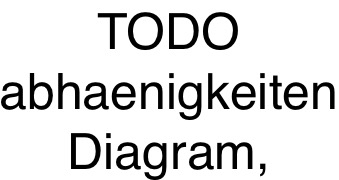
\includegraphics[width=0.95\textwidth]{graphics/abhaengigkeiten}
    \caption{Strukturelle Abhängigkeiten der projektinternen Rust-Crates}
    \label{fig:crate-abhaengigkeiten}
\end{figure}





\subsection{Gemeinsame Datenstrukturen und Map-ABI}
Die eBPF-Maps bilden die gemeinsame Datenschnittstelle zwischen Userspace und Kernelspace. Sie speichern Schlüssel und Werte als Bytefolgen, denen keine Rust-Typinformationen beigefügt sind. Damit ein im Userspace geschriebener Map-Eintrag vom eBPF-Programm eindeutig gelesen werden kann, müssen beide Ausführungsbereiche dieselbe Binärrepräsentation der verwendeten Datenstrukturen zugrunde legen. Dies betrifft insbesondere Feldreihenfolge, Feldgrößen und Ausrichtung der Schlüssel und Werte.

Diese gemeinsame Repräsentation bildet die Map-ABI des Prototyps. Die hierfür benötigten Strukturen sind in \path{tails-pdp-common} gebündelt und werden sowohl vom eBPF-Programm als auch von den Userspace-Komponenten verwendet. Die folgenden Unterabschnitte beschreiben die kernelgeeignete Darstellung von Policies und Attributen, die Identifikation von Ressourcen in Map-Schlüsseln sowie Aufbau und Pinning der verwendeten Maps. Das Einlesen, Validieren und Übersetzen der Policy- und Attributdateien wird dagegen in den nachfolgenden Abschnitten behandelt.

\subsubsection{Kernelgeeignete Policy-Strukturen}
Die Policy-Repräsentation ist auf eine konstante Größe und einen vorhersehbaren Kontrollfluss im eBPF-Programm ausgelegt. Für den Hook \texttt{file\_open} existieren deshalb getrennte Strukturen für statische und attributabhängige Policies. Beide Varianten enthalten die Zugriffsentscheidung, die Aktion, einen Aktivierungsstatus, das Subject sowie die Bedingungen für Kommando und Ressource. Kommando- und Ressourcenbezeichnungen werden dabei nicht als dynamische Zeichenketten, sondern als Arrays fester Länge abgelegt. Für Ressourcen werden zusätzlich Device- und Inode-Wert gespeichert.

Die Struktur \texttt{FileOpenStaticPolicy} enthält nur die Bedingungen, die unmittelbar mit dem Öffnungsvorgang verglichen werden können. \texttt{FileOpenStreamPolicy} erweitert diese Repräsentation um eine optionale Zeitbedingung und ein fest dimensioniertes Feld für Attributbedingungen. Jede dieser Bedingungen besteht aus Namespace, Vergleichsoperator, Werttyp, Hash des Attributnamens und dem Vergleichswert. Die Anzahl der aktiven Bedingungen wird gesondert gespeichert; das zugrunde liegende Array besitzt dennoch stets eine feste Obergrenze von vier Einträgen. Damit kann die Auswertung im eBPF-Programm mit begrenzten Schleifen erfolgen, ohne Speicher dynamisch reservieren zu müssen.

Beide Policy-Typen werden als Werte separater Array-Maps gespeichert. Nicht belegte Einträge werden mit einer deaktivierten Policy gefüllt. Die Trennung in statische und attributabhängige Policies erlaubt es, die Auswertung in getrennten Tail-Call-Stufen auszuführen. Die konkrete Aktivierung einer vollständigen Policy-Generation wird in Abschnitt~\ref{sec:policy-generation} beschrieben.

\subsubsection{Repräsentation dynamischer Attribute}
Das Attributmodell muss frei wählbare Namen und Werte abbilden, obwohl eBPF-Maps nur Strukturen fester Größe speichern können. Ein Attribut wird deshalb durch einen festen Schlüssel und einen typisierten Wert repräsentiert. \texttt{AttributeKey} enthält die aktive Attributbank, den Namespace, zwei Objektidentifikatoren und einen 128-Bit-Hash des Attributnamens. Der Schlüssel legt damit fest, zu welchem System-, Subject- oder Ressourcenobjekt ein Attribut gehört und unter welchem Namen es angesprochen wird.

\texttt{AttributeValue} unterscheidet numerische, boolesche und Zeichenkettenwerte. Zahlen und Wahrheitswerte werden direkt als \texttt{u64} gespeichert. Für Zeichenketten wird nicht der Text selbst, sondern sein 128-Bit-Hash abgelegt. Der Userspace validiert Attributnamen vor der Übernahme und akzeptiert ausschließlich ASCII-Buchstaben, Ziffern, Unterstriche und Bindestriche. Anschließend werden Name und gegebenenfalls Zeichenkettenwert mit derselben Hashfunktion in die feste Kernelrepräsentation übersetzt. Der Kernel muss daher weder Zeichenketten parsen noch dynamischen Speicher verwalten.

Die Policy-Struktur enthält zu jeder Attributbedingung denselben Namenshash sowie den erwarteten Wert. Bei der Auswertung erzeugt das eBPF-Programm aus der aktuellen Attributbank, dem Namespace und der Objektidentität einen \texttt{AttributeKey} und liest den zugehörigen Wert aus der Hash-Map. Fehlt ein erforderliches Attribut oder stimmt sein Typ beziehungsweise Vergleichswert nicht überein, gilt die Bedingung als nicht erfüllt. Details zum Einlesen und Validieren der \path{.attributes}-Dateien behandelt Abschnitt~\ref{sec:attribute-loading}.

\subsubsection{Objektidentitäten im Map-Schlüssel}
Die beiden Objektidentifikatoren im Attributschlüssel werden abhängig vom Namespace belegt. Für Systemattribute sind beide Werte null, da sie systemweit gelten. Subject-Attribute verwenden die numerische UID als primären Identifikator; der zweite Wert bleibt null. Ressourcenattribute verwenden dagegen Device- und Inode-Wert der Datei. Diese Zuordnung wird sowohl beim Einlesen der Attributdateien im Userspace als auch bei der eBPF-Auswertung verwendet.

Die Ressourcenidentität wird aus den Dateimetadaten ermittelt, nicht aus dem Pfadnamen. Der Pfad dient beim Attributloader lediglich dazu, die zugehörige Datei zu finden und ihre Metadaten auszulesen. In der Map werden Device und Inode als zwei getrennte \texttt{u64}-Werte gespeichert. Dadurch wird keine verkürzende Hash-Repräsentation der Ressourcenidentität verwendet und Dateien auf unterschiedlichen Dateisystemen bleiben unterscheidbar. Zugleich bleibt die Zuordnung bei Umbenennungen derselben Datei erhalten, solange Device und Inode unverändert bleiben.

Die Objektidentität ist Teil des Map-Schlüssels und damit Teil der ABI. Eine Änderung ihrer Größe, Reihenfolge oder Bedeutung würde den Aufbau der \path{ATTRIBUTES}-Map verändern. Bereits gepinnte Maps wären dann nicht mehr kompatibel und müssen vor dem Laden eines Programms mit dem geänderten Layout erkannt werden.

\subsubsection{Aufbau und Pinning der eBPF-Maps}
Tabelle~\ref{tab:pinned-map-abi} zeigt die gepinnten Maps, die den dauerhaften Datenaustausch zwischen den Komponenten ermöglichen. Die Policy- und Attributloader schreiben gültige Daten in diese Maps. Das eBPF-Programm liest sie bei der Zugriffsentscheidung; Userspace-PEP und Administrationstool öffnen dieselben Maps bei Bedarf erneut zur Überwachung beziehungsweise Anzeige.

\begin{table}[htbp]
    \centering
    \small
    \begin{tabular}{|p{4.2cm}|p{1.7cm}|p{3.4cm}|p{4.4cm}|}
        \hline
        \textbf{Map} & \textbf{Typ} & \textbf{Schlüssel und Wert} & \textbf{Aufgabe} \\
        \hline
        {\scriptsize\texttt{POLICY\_GENERATION}} & Array & \texttt{u32} $\rightarrow$ \texttt{u32} & Speichert die aktive Policy-Generation und bestimmt damit die auszuwertende Policy-Bank. \\
        \hline
        {\scriptsize\texttt{FILE\_OPEN\_STATIC\_POLICIES}} & Array & \texttt{u32} $\rightarrow$\newline {\scriptsize\texttt{FileOpenStaticPolicy}} & Enthält die statischen \texttt{file\_open}-Policies beider Policy-Banken. \\
        \hline
        {\scriptsize\texttt{FILE\_OPEN\_STREAM\_POLICIES}} & Array & \texttt{u32} $\rightarrow$\newline {\scriptsize\texttt{FileOpenStreamPolicy}} & Enthält die attribut- und zeitabhängigen \texttt{file\_open}-Policies beider Policy-Banken. \\
        \hline
        {\scriptsize\texttt{CURRENT\_TIME}} & Array & \texttt{u32} $\rightarrow$ \texttt{u64} & Stellt den aktuellen Unix-Zeitstempel für zeitabhängige Bedingungen bereit. \\
        \hline
        {\scriptsize\texttt{ATTRIBUTE\_GENERATION}} & Array & \texttt{u32} $\rightarrow$ \texttt{u32} & Speichert die aktive Attributgeneration und damit die aktive Attributbank. \\
        \hline
        {\scriptsize\texttt{ATTRIBUTES}} & Hash-Map & {\scriptsize\texttt{AttributeKey}} $\rightarrow$\newline {\scriptsize\texttt{AttributeValue}} & Enthält die dynamischen System-, Subject- und Ressourcenattribute. \\
        \hline
    \end{tabular}
    \caption{Gepinnte eBPF-Maps als Map-ABI des Prototyps}
    \label{tab:pinned-map-abi}
\end{table}

Beim Start legt \texttt{tails-pdp} das Pin-Verzeichnis \path{/sys/fs/bpf/tails-pdp} an und lädt das eBPF-Objekt mit diesem Verzeichnis als Standardpfad für Maps. Gepinnte Maps bleiben im BPF-Dateisystem erreichbar und können deshalb von später gestarteten Userspace-Komponenten über ihren Pfad geöffnet werden. Die nicht gepinnten Maps für Tail Calls, temporäre Entscheidungen und Debug-Konfiguration gehören dagegen ausschließlich zum geladenen eBPF-Objekt und sind nicht Teil der gemeinsamen Map-ABI.

Da gepinnte Maps einen Programmneustart überdauern können, prüft \texttt{tails-pdp} vor dem Laden des eBPF-Programms vorhandene Map-Layouts. Für jede ABI-relevante Map werden Schlüsselgröße, Wertgröße und maximale Eintragszahl mit den aktuellen Strukturdefinitionen verglichen. Bei einer Abweichung wird der Start abgebrochen, statt eine vorhandene Map mit einer möglicherweise falsch interpretierten Byte-Repräsentation weiterzuverwenden. Die Generationswechsel für Policies und Attribute bauen auf diesen stabilen Map-Layouts auf und werden in den jeweiligen Verarbeitungsabschnitten erläutert.

\subsection{Initialisierung und Laufzeitsteuerung}
\subsubsection{Laden und Prüfen des eBPF-Programms}
\subsubsection{Initialisierung der Maps und Tail Calls}
\subsubsection{Start der Userspace-Komponenten}

\subsection{Verarbeitung und Laden von Policies}
\subsubsection{Einlesen der Policydateien}
\subsubsection{Syntaktische Verarbeitung}
\subsubsection{Semantische Validierung}
\subsubsection{Übersetzung in Map-Einträge}
\subsubsection{Generationenwechsel und Rollback}\label{sec:policy-generation}

\subsection{Bereitstellung dynamischer Attribute}\label{sec:attribute-loading}
\subsubsection{Aufbau des Attributverzeichnisses}
\subsubsection{Parsen und Validieren der Attribute}
\subsubsection{Attributschlüssel und Hashwerte}
\subsubsection{Aktualisierung der Attributgeneration}
\subsubsection{Bereitstellung der Zeitinformation}

\subsection{Implementierung des Kernelspace-PEP}
\subsubsection{Verarbeitung des file\_open-Hooks}
\subsubsection{Tail-Call-Kette}
\subsubsection{Auswertung statischer Policies}
\subsubsection{Auswertung von Streampolicies}
\subsubsection{Combining und Durchsetzung}

\subsection{Implementierung des Userspace-PEP}
\subsubsection{Ermittlung bestehender Dateizugriffe}
\subsubsection{Erneute Policy-Auswertung}
\subsubsection{Entzug des betroffenen File Descriptors}

\subsection{Implementierung des Administrationstools}

\subsection{Fehlerbehandlung und Konsistenzsicherung}

\subsection{Build und Deployment auf dem Zielsystem}
\subsubsection{Cross-Compilation und Build-Artefakte}
\subsubsection{Implementierungsbedingte Grenzen}

\newpage
